\chapter{SIGNAL AND BACKGROUND MODELS FOR THE $H\rightarrow\mu^+\mu^-$ SEARCH} \label{modeling}

This chapter presents the signal and background modeling for the $H\rightarrow\mu^+\mu^-$ search. The signal MC samples are fit to model the signal, and the data is fit to model the background. The systematic uncertainties and the evaluation of the background for bias are covered in Section \ref{unc}.

%%%%%%%%%%%%%%%%%%%%%%%%%%%%%%%%%%%%%%%%%%%%%%%%%%%%%%%
\section{Modeling The Signal}
The signal in the $H\rightarrow\mu^+\mu^-$ search is a peak in the $m_{\mu\mu}$ spectrum, and it is modeled by fitting the signal MC after corrections, event selection, and categorization. The PDFs for the GGF, VBF, ZH, $W^+H$, $W^-H$, and $t\bar{t}H$ processes are fit separately, and the net PDF for the signal is the sum of the individual PDFs. The signal for each process in each category is fit with the same parametric form, a triple Gaussian\footnote{Three of the process, category fits have very low stats and use only two Gaussians.}, 
\begin{equation}
\label{eq:sigpdf}
S_{pc}(x, m_H, \theta_{pc}) = \sum_{g=1}^{3}f_{pcg}\mathcal{N}(x, \mu_{pcg}, \sigma_{pci}).
\end{equation}
In \ref{eq:sigpdf}, x runs along $m_{\mu\mu}$, p labels the signal process, c labels the category, g labels the Gaussian, and $\mathcal{N}(x, \mu, \sigma)$ is a Gaussian with mean $\mu$ and width $\sigma$. One Gaussian picks up the peak at the center, another wider Gaussian fits the remaining width at the core, and the final Gaussian accounts for the slightly higher probability in the low mass tail. Energy loss effects like Final State Radiation (FSR) and brehmsstrahlung increase the probability to measure a lower than average Higgs mass. 

The PDFs for the signal in each category are fit at $m_H$ = 120, 125, and 130 GeV, using the signal MC at those masses. To get the signal PDFs for any $m_H$ value in the [120, 130] GeV search window, the fit parameters are interpolated (linearly) between the best fit values at 120, 125, and 130 GeV. Figure~\ref{sigmodel:gaus} shows an example of a fit on the left, its interpolation in the center, and the efficiency times acceptance on the right.

\begin{figure}[h!]
    \centering
    \includegraphics[width=0.3\textwidth]{images/signal_model_updated/ggf/fit_mh_125_GluGlu_cat3_NEW.png}
    \includegraphics[width=0.3\textwidth]{images/signal_model_updated/interp_and_norm/interpolation_GluGlu_cat3_NEW.png}
    \includegraphics[width=0.3\textwidth]{images/signal_model_updated/interp_and_norm/norm_GluGlu_cat3_NEW.png}
    \caption[An example of the signal model.]
    {An example Higgs signal fit for a specific production
    process and category at a mass of 125~GeV (left), its
    interpolation to lower and higher mass (center), and its efficiency times
    acceptance vs $m_H$ (right).}
    \label{sigmodel:gaus}
\end{figure}
The PDFs describe the shape of the signal distribution, but not the total number of signal events. The models describing the signal yields are determined by normalizing the PDFs to the expected SM yields. 
\begin{align}
        %\label{eq:signalNormalization}
        %\text{Norm} = {\frac{\mathcal{L} \sigma \mathcal{B}(\Htomm)}{N_{gen}}} \\
        \label{eq:expectedYield}
        %\text{Yield} = {Norm \times \sum_{bins}^{} N_{i}}
        %\label{eq:efficienceAcceptance}
        \text{Yield}_{pc} = \mathcal{L}\,\sigma(pp\rightarrow H)\, \mathcal{B}(H\rightarrow\mu^+\mu^-) \, \varepsilon_{pc}A_{pc}
\end{align}
$\mathcal{L}\sigma(pp\rightarrow H)\mathcal{B}(H\rightarrow\mu^+\mu^-)$ provides the total number of $H\rightarrow\mu^+\mu^-$ events expected by the SM, and the efficiency times acceptance, $\varepsilon_{pc} A_{pc}$, provides the fraction expected for the given process in the given category, 
\begin{align}
\varepsilon_{pc} A_{pc} = \frac{1}{N}\sum_{i \in p} w_{i} \cdot r_{i} \cdot \text{sf}_i \cdot \mathbf{I}\{i \in c\}.
\end{align}
The sum runs over all MC events for the signal process. The factors $w_i$, $r_i$, and $sf_i$ are the MC weight, the PU reweighting factor, and the scale factor for the event, respectively. The indicator function, $\mathbf{I}\{i \in c\}$, is 0 if the event i is not in the category and 1 if it is. The normalization, N, is given by the sum of MC weights over all the signal processes, $\sum_{i}w_{i}$. The cross section, $\sigma(pp\rightarrow H)$, and branching fraction, $\mathcal{B}(H\rightarrow\mu^+\mu^-)$, are taken from the Yellow Report 4, and provided centrally by combine.

The left side of Figure~\ref{sigmodel:all} shows the sum of the signal models over all processess and categories. The right side of the figure shows the net signal for one of the best mass resolution categories. The plots are divided by the number of expected events, $\mathcal{L}\sigma\mathcal{B}$, to present the fraction of signal expected per GeV, rather than the net yield per GeV. The blue line represents the sum of the fits and the points represent the MC predictions. 
\begin{figure}[h!]
    \centering
    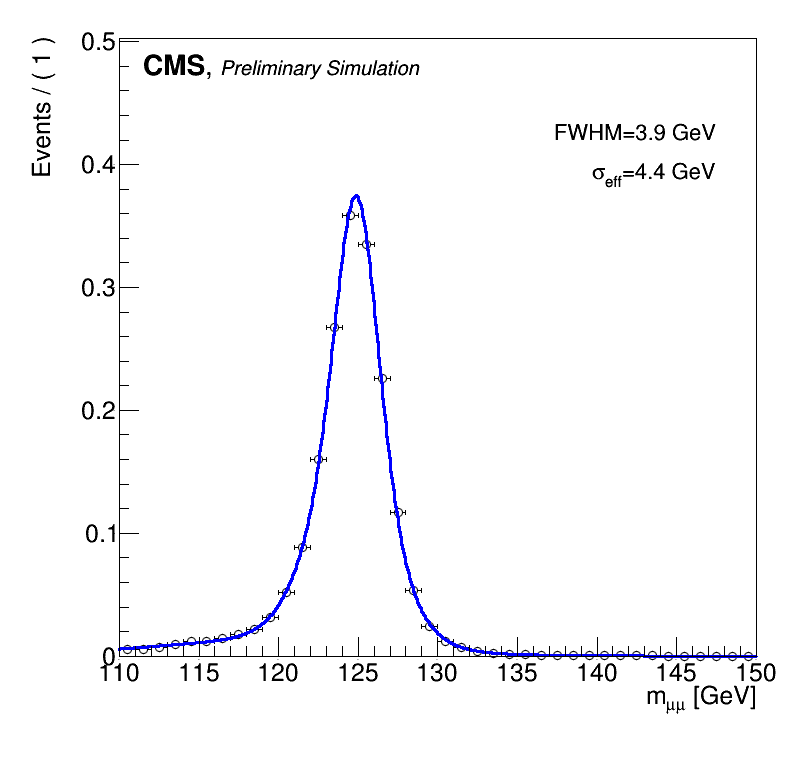
\includegraphics[width=0.49\textwidth]{images/signal_model_updated/net/signal_model_all.png}
    \includegraphics[width=0.49\textwidth]{images/signal_model_updated/net/signal_model_cat3_NEW.png}
    \caption[The signal model compared to MC predictions.]
    {Signal model compared to MC predictions, summing up the contribution from all process and all categories (left), and for one of the categories with the best mass resolution.}
    \label{sigmodel:all}
\end{figure}
Figure~\ref{sigmodel:comp} shows the composition of the signal model, the mass resolution, and the S/(S+B) in each category.
\begin{figure}[h!]
    \centering
    \includegraphics[width=0.99\textwidth]{images/signal_model_updated/signal_composition_small.png}
    \caption[The signal composition, resolution, and purity in the different categories.]
    {The signal composition, the mass resolution in Half Width Half Max ($\sigma_{HM}$) and 68\% probability ($\sigma_{eff}$), and the S/(S+B) of the different categories.}
    \label{sigmodel:comp}
\end{figure}
Figure~\ref{sigmodel:effacc} shows the efficiency times acceptance of the selection --  prior to categorization -- for the total signal and for each signal process.
\begin{figure}[h!]
    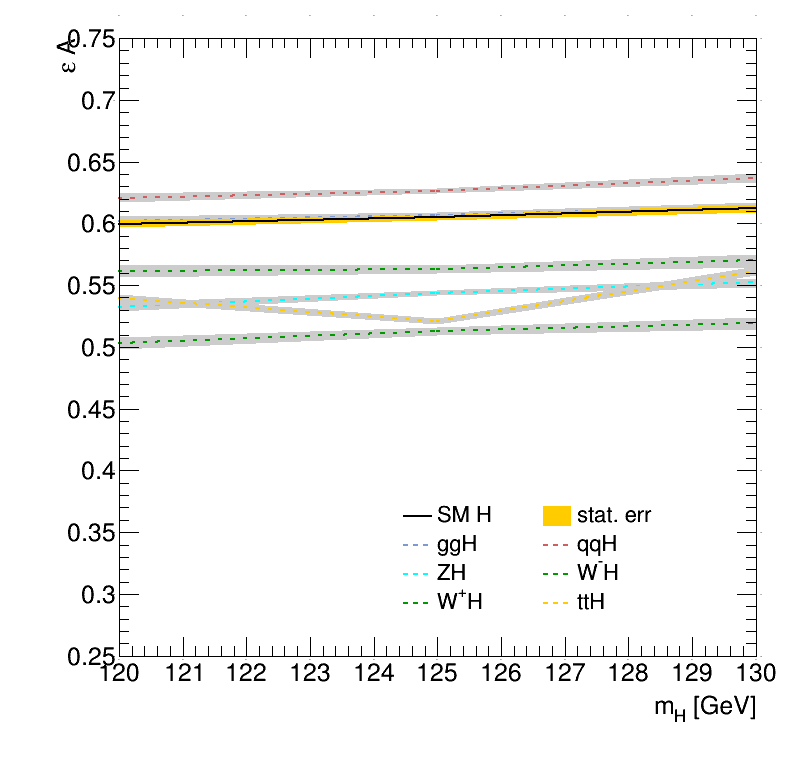
\includegraphics[width=0.79\textwidth]{images/signal_model_updated/effAcc.png}
    \caption[The efficiency times acceptance versus the Higgs mass.]
    {The efficiency times acceptance as function of $m_H$ for the total signal and for each signal process.}
    \label{sigmodel:effacc}
\end{figure}
%%%%%%%%%%%%%%%%%%%%%%%%%%%%%%%%%%%%%%%%%%%%%%%%%%%%%%%
\section{Modeling The Background}

The background for $H\rightarrow\mu^+\mu^-$ is a smoothly falling spectrum in $m_{\mu\mu}$ dominated by Drell-Yan and $t\bar{t}$. The background in the signal region, 120 to 130 GeV, is estimated by fitting the data in the sidebands, $[110, 120) \cup (130,150]$ GeV. While MC samples are available for the background, fitting the data provides a much better estimate. First, the data collected far exceeds the amount of MC available, and the larger statistics in data provide a reduced uncertainty on the estimated background. Second, the MC has many additional uncertainties like those from higher order QCD and EW contributions, resummation effects, and estimates of the parton density function, among others. With a lower the uncertainty on the estimated background, it's easier to tell a signal peak from a background fluctuation. 

In order to find an accurate background fit with the lowest uncertainty, many different models are studied. The models are organized into three classes. The first class is physically motivated, using analytic functions based upon the Breit-Wigner for the Z peak. The functions modify the Breit-Wigner to control the decay at large mass where $t\bar{t}$ kicks in. 
\begin{align}
        %\label{eq:ExpPol2}
        %\text{ExpPolynomial: }& {B(x)} = {e^{a_{1}x + a_{2}x^2}} \\
        \label{eq:BWZ}
        \text{BWZ: }& {B(x)} = {\frac{e^{ax}\sigma_{z}}{(x-\mu_{z})^2 + (\frac{\sigma_{z}}{2})^2}} \\
        \label{eq:BWZRedux}
        \text{BWZRedux: }& {B(x)} = {\frac{e^{a_{2}x + a_{3}x^2}}{(x-\mu_{z})^{a_{1}} + (\frac{2.5}{2})^{a_{1}}}} \\
        \label{eq:BWZGamma}
        \text{BWZGamma: }& {B(x)} = {f\frac{e^{ax}\sigma_{z}}{(x-\mu_{z})^2 + (\frac{\sigma_{z}}{2})^2} + (1-f)\frac{e^{ax}}{x^2}}
\end{align}
These models have been validated by fitting the FEWZ (NNLO QCD) generated mass shapes and by fitting the data in the sidebands. The second class of models are the FEWZ shapes of the DY spectrum for the fully inclusive spectrum (NNLO), DY with one jet (NLO), and DY with two jets (LO). The FEWZ shapes are implemented as splines of the FEWZ histograms modulated by Bernstein polynomials in the same way as Equation \ref{eq:BWZReduxPoly}. The polynomials multiplying the theoretical FEWZ shapes account for resolution smearing effects and the contributions from backgrounds besides DY. The third class are the general purpose functions, which can fit any smoothly falling background with enough terms.
\begin{align}
        \label{eq:Bernstein}
        \text{Bernstein: }& {B(x)} = {\sum_{i=0}^{n} \alpha_i[\binom{n}{i}x^{i}(1-x)^{n-i}}] \\
        \label{eq:SumExponentials}
        \text{SumExponentials: }& {B(x)} = {\sum_{i=1}^{n} \beta_{i}e^{\alpha_{i}x}}
        %%\text{SumPowers:}& {B(x)} = {\sum_{i=1}^{n} \beta_{i}x^{\alpha_{i}}}\\
        %%\label{eq:SumPowers}
        %%\text{LaurentSeries:}& {B(x)} = {\sum_{i} \alpha_{i}x^{i}}
        %%\label{eq:Laurent}
\end{align}
The analysis also uses a modified version of the BWZRedux ($BWZR(x)$, Eq.~\ref{eq:BWZRedux}) modulated by a Bernstein polynomial of degree $n$ ($BERN(x,n)$, Eq.\ref{eq:Bernstein}, normalized to $1$):
\begin{align}
        \label{eq:BWZReduxPoly}
        \text{BWZRedux}\cdot\text{Bern: }& {B(x)} = BWZR(x) \cdot \left(1+ BERN(n,x)\right) \\
\end{align}
The modulated BWZRedux makes the model more flexible and helps to reduce any bias that may exist towards the unknown underlying true distribution.
\begin{figure}[hbp]
     \centering
     \includegraphics[width=0.3\textwidth]{images/background_model/baseline_p25GeV_110to160/backgroundFits__01JetsTightBB__bkgModels.png}
     \includegraphics[width=0.3\textwidth]{images/background_model/baseline_p25GeV_110to200/backgroundFits__01JetsTightBB__bkgModels.png}
     \includegraphics[width=0.3\textwidth]{images/background_model/baseline_p25GeV_110to250/backgroundFits__01JetsTightBB__bkgModels.png}
     \caption[Some background-only fits.]
     {Example background-only fits to the dimuon mass spectrum in data for various background models and mass ranges.}
     \label{bkgmodel:exampleModels}
\end{figure}

For each category, the order of each FEWZ shape and of each general purpose function is selected using the F-Test method at 95\% CL. The method is described in detail below.
\begin{itemize}
%    \item for a given category and for a particular family
    \item Null hypothesis: There is no difference between orders $n$ and $n+1$.
    \item If there is no difference, the likelihoods for the two models will show little difference in goodness of fit on the data.
    \item To reject this hypothesis at 95\% confidence, the p-value for 2$\Delta N_{LL}$ must be less than 5\%, $p-\text{value}(\chi^2, ndf) < 5\%$.
    \item Perform the background only fit to the data for orders $n$ and $n+1$.
    \item Use $\chi^2 = -2\Delta\log\mathcal{L}$ using the asymptotic approximation of the Likelihood function.
    \item Compute the difference in number of degrees of freedom $\text{n.d.f.} = \text{NDF}_{n+1} - \text{NDF}_{n}$.
    \item The $\chi^2$ variable is distributed as a $\chi^2$-distribution with $\text{n.d.f.}$ degrees of freedom.
    \item Compute the $\chi^2$ p-value.
    \item For a p-value less than $5\%$, reject n and move on to test n+1.
    \item For a p-value greater than $5\%$, we stop and select order $n$ for this category, for this functional family.
\end{itemize}
Figure~\ref{bkgmodel:exampleFTest} shows an example of the F-Test for the Bernstein Polynomials and for the Sum of Exponentials.
\begin{figure}[hbp]
     \centering
     \includegraphics[width=0.45\textwidth]{images/background_model/baseline_ftest_p25GeV_110to160/ftest__01JetsTightBB__bernsteinFastModels.png}
     \includegraphics[width=0.45\textwidth]{images/background_model/baseline_ftest_p25GeV_110to160/ftest__01JetsTightBB__sumExpModels.png}
     \caption[An example of the F-Test for the ordered background fits.]
     {Examples of the F-Test for the Bernstein Polynomials (left) and the Sum of Exponentials (right).}
     \label{bkgmodel:exampleFTest}
\end{figure}

%%%%%%%%%%%%%%%%%%%%%%%%%%%%%%%%%%%%%%%%%%%%%%%%%%%%%%%
\section{Systematic Uncertainties} \label{unc}
In order to report accurate results, it's essential to incorporate all known uncertainties affecting the signal and background models. These so-called "systematics" broaden the likelihood's PDF, worsen the limits, and increase the uncertainty of the measurement. The known contributions for the signal model are covered in the next section, and the background uncertainties are covered after. 
%%%%%%%%%%%%%%%%%%%%%%%%%%%%%%%%%%%%%%%%%%%%%%%%%%%%%%%
\subsection{Signal}
The uncertainties on the signal model are broken down into shape, category migration, and rate uncertainties. Shape uncertainties affect the shape of the signal PDF. Category migration uncertainties quantify the migration of signal events from one category to another, and rate uncertainties affect the total number of $H\rightarrow\mu^+\mu^-$ events expected. The WG1 uncertainties on GGF affect all three, and these are mentioned in the rate uncertainty section. A quantitative comparison of the different uncertainties is outlined in the impacts plot, Figure \ref{fig:impacts}. 

\subsubsection{Shape uncertainties}
The shape of the $m_{\mu\mu}$ signal peak is determined by the $p_t$, $\eta$, and $\phi$ measurements for the muons. The centrally provided Kalman Filter muon momentum corrections provide uncertainties on the muon momenta in terms of the scale and resolution. The muon $\eta$ and $\phi$ measurements are precise enough to be neglected in comparison.

\begin{itemize}
    \item {\bf Muon Scale} The scale of the momentum affects the position of the $m_{\mu\mu}$ peak, and propagating this uncertainty to the mass shifts the signal peak a maximum of 0.05\%. A single nuisance is used to quantify the scale uncertainty, correlated acrosss the cateogories.
    \item {\bf Muon Resolution} The resolution affects the width of the peak and propagating this uncertainty to the mass affects the width of the signal peak up to 10\%. Again, a single nuisance is used correlated across the categories.
\end{itemize}

\subsubsection{Category migration uncertainties}
Moving the values of certain factors in the analysis may cause a signal event to migrate from one category to another affecting the yields in the categories. The uncertainties in these factors therefore affect the uncertainty of the yields across the categories. The major migration uncertainties are discussed below.  

\begin{itemize}
    \item {\bf Jet Energy Scale} After applying the jet energy corrections {\it Summer16\_23Sep2016AllV4}, the energy scale of
    the jet is varied as provided by the JetMET group. The variation shifts the jet energy and propagates the shift to the MET for the event. 
    The jet energy variations lead to variations in category yields, especially in the high sensitivity VBF-like categories.
    The jet energy scale is the dominant experimental uncertainty with up to $6\%$ variation in the yields and the largest impact on the signal strength measurement.
    The effect of the scale uncertainty can be seen in the error bands in Fig.~\ref{fig:jes}, 
    showing coverage for data/MC discrepancies in jet eta and the number of jets.
    \item {\bf Jet Energy Resolution} The uncertainty in jet energy resolution also causes category migrations. 
    Upon widening the resolution, events migrate along the steeply falling $p_t$ spectrum. 
    More events move from the highly populated low $p_t$ regime into the less populated high $p_t$ regime, causing events to move between categories. 
    The resolution uncertainty leads to variations in the yields up to 3\%.
    \item {\bf Pile-up Re-weighting} The pile-up re-weighting procedure uses the minimum bias cross section to 
    estimate the amount of pile-up in data. The amount of Pile-up has two major effects. First, it can reduce the efficiency of
    the muon selection by increasing the nearby hadronic activity, and, second, it may create random clusters of energy that become identified as jets.
    But thanks to the PU removal techniques in the jet reconstruction and muon isolation, the PU uncertainty only leads to $1\%$ variations in the signal yield.
    \item {\bf b-jet Efficiency} The uncertainty in the b-tagging efficiency also leads to yield variations, but due to the fact that b-jets are 
    vetoed in the most sensitive categories to suppress the {$t\bar{t}$}, the uncertainty yields $\simeq 1\%$ variations.
    \item {\bf b-jet Fake Rate}  Same as above but correcting the efficiency of light-flavored jets to fake a b-jet ($\simeq 1\%$).
    \item {\bf MC R/F Scale} Varying the renormalization and factorization scales up and down by a factor $2$, yields up to $\simeq 6\%$ migration.
    The contribution to the total signal yield is described in the next section on rate uncertainties.
    \item {\bf MC PDF} Parton distribution functions are varied using the NNPDF3.0 weights available in the production. 
    These variations amount to $\simeq 2/3\%$ signal yield variation. The contribution to the total sample normalization is covered in the 
    next section on rate uncertainties.
    \item {\bf MC Tune} Tune uncertainty is derived using the centrally provided up and down MC variations of the MC tune for pythia8.
    \item {\bf Parton Shower} Parton Shower uncertainty is derived using the centrally produced up and down MC variations of the pythia8 showering settings.
\end{itemize}

\begin{figure}[h!]
    \centering
    \includegraphics[width=0.49\textwidth]{images/sig_syst/EtaJet1OnH_bkg}
    \includegraphics[width=0.49\textwidth]{images/sig_syst/NJetsOnH_bkg}
    \caption[Uncertainty on some jet kinematics and counts.]
    {Pseudorapidity of the leading jet, and number of associated jets. The uncertainty bands show jet energy scale uncertainty.}
    \label{fig:jes}
\end{figure}

\subsubsection{Rate uncertainties}
Rate uncertainties affect the total number of SM $H\rightarrow\mu^+\mu^-$ events expected. The theoretical uncertainties include those on the branching fraction and the signal production cross section. The experimental uncertainties include those on the luminosity and the muon scale factors.  

\begin{itemize}
    \item {\bf $H\rightarrow\mu^+\mu^-$ Branching Fraction} The branching fraction has an uncertainty of $1.7\%$ and applies to all signal production.
    \item {\bf R/F -- Cross Section} The GGH cross section has an uncertainty of $3.9\%$ due to renormalization and factorization (R/F), 
    VBF $0.4\%$, ZH $3.8\%$, WH $0.6\%$, and $t\bar{t}H$ $-9.9\%$ to $+6.8\%$.
    \item {\bf PDF -- Cross Section} The parton distribution function contributes an uncertainty of $3.2\%$ to the GGH cross section, 
    $2.1\%$ to VBF, $1.6\%$ to ZH, $1.9\%$ to WH, and $3.7\%$ to $t\bar{t}H$.
    \item {\bf WG1 uncertainties} Additional uncertainties on GGF are applied using the WG1 recommendations.
    These apply uncertainties ontop of the R/F and PDF uncertainties accounting for different effects like the
    uncertainty in yield over jet $p_t$, the number of jets, and other factors.  
    The WG1 corrections affect the shape, category migration, and rate. 
    These are marked THU in the impact assessment of Figure \ref{fig:impacts}. 
    \item {\bf Luminosity} The luminosity measurement has an uncertainty of $2.5\%$.
    \item {\bf Muon Scale Factors} The muon scale factors provided by
      the POG have an uncertainty of $0.5\%$ for the trigger, $1.0\%$ for the muon ID, and $0.5\%$ for the isolation. 
      Uncertainties on the different runs are taken to be correlated.
\end{itemize}

\subsubsection{Impact plots}
The influence of the different uncertainties on the signal strength measurement are shown in Fig.~\ref{fig:impacts}. The uncertainties are sorted in decreasing order of their impact, $\Delta\hat{\mu}$, induced by a $\pm1\sigma$ variation of the systematic under evaluation.

\begin{figure}[h!]
    \centering
    \includegraphics[width=0.85\textwidth]{images/sig_syst/impacts.pdf}
    \caption[Impact plots using the Asimov dataset.]
    {Impact plots derived from the Asimov dataset.}
    \label{fig:impacts}
\end{figure}

\FloatBarrier
\subsection{Background}
The background is modeled by fitting the data, and the likelihood from the fit naturally accounts for the uncertainties in the fit parameters leaving fewer systematics to incorporate as additional constraints. Unfortunately, when using an arbitrary model to estimate the background it is unknown whether the form of the model can accurately fit the underlying true distribution in each of the categories. If the model cannot accurately fit the underlying true distribution, then the signal measured will differ from the truth and the model is "biased". In order to report accurate results it is therefore important to assess the existence of any bias, and account for it appropriately. 

To quantify the bias of a particular model, the following process is used. The analysis chooses a set of reasonable models $\beta = {B_1, B_2, B_3, ..., B_N}$. Then the bias of model $B_i$ towards hypothesis $B_j$ is evaluated by assuming that $B_j$ is the underlying true model. $B_j$ is fit to the sidebands in data, and the best fit for $B_j$ is used along with the signal model to form the S+$B_j$ PDF, emulating a world where S+$B_j$ represents the truth. This PDF is used to generate pseudodata at the given integrated luminosity with a signal strength ($\mu$, sometimes called r) of 1 representing the SM. The pseudodata is fit in the sidebands with $B_i$ and the best fit of the signal strength ($\hat{\mu}_{ij}$) is determined. With a true $\mu$ of one the expected $\hat{\mu}_{ij}$ should be 1. To get a distribution for $\hat{\mu}_{ij}$, the pseudodata is generated by S+$B_j$ and fit by S+$B_i$ to extract $\hat{\mu}_{ij}$. If the median $\hat{\mu}_{ij}$ is not 1 then $B_{i}$ is biased towards $B_{j}$. As such, the bias is defined to be,
\begin{equation}
b_{ij} = Median\left[\frac{\hat{\mu}_{ij} - \mu}{\sigma_{\mu,ij}}\right]
\end{equation}
with $\mu=1$. $B_i$ is unbiased towards $B_j$ if $b_{ij}$ is close to zero. The median is taken over 2500 trials yielding an uncertainty in $b_{ij}$ of about $2\%$. The bias for all $B_i \in \beta$ is evaluated for all $B_j \in \beta$, providing the NxN matrix $b$. 

If a bias is found, the background model tends to under or over estimate the background and measure too much or too little signal. When this is the case, a "spurious signal" is added to the background model to compensate. The spurious signal has the same shape as the signal model, with a normalization constrained by a Gaussian with mean 0 and $\sigma = b_{ij}\sigma_{\mu}N$, where N is the expected number of signal events in the category. The spurious signal allows the background more freedom in the signal region, fixing the tendency to mismeasure the signal. On the other hand, this added freedom in the signal region increases the background uncertainty there, reducing the sensitivity. 

A bias less than 0.20 has a negligible effect on the upper limits ($<2\%$). In this case, the spurious signal can usually be neglected. With this information, the analysis attempts to find fits for each category such that the maximum likelihood estimate of $\mu$ is unbiased ($b_{ij} < 0.20$) with respect to all $B_j \in \beta$. The bias matrices for $m_H=125 GeV$ are shown in Figures \ref{fig:bias_1} and \ref{fig:bias_2}. The matrices present the bias towards $\hat{\mu}$ for the category's likelihood alone and zero spurious signal. 

The set of reasonable functions used is $\beta = \{BWZRedux\cdot poly, BWZGamma,$ 
$SumExp, FEWZ-full\cdot poly, FEWZ-1-jet\cdot poly, FEWZ-2-jet\cdot poly\}$. Polynomial orders 0-4 are examined for BWZRedux$\cdot$poly, and the F-Test at 95\% confidence is used to select the orders for SumExp and the FEWZ$\cdot$poly models. The Bernstein polynomials proved biased towards all of the other functions, so they are considered unreasonable and excluded from $\beta$. 
\begin{figure}[h!]
    \centering
    \includegraphics[width=0.32\textwidth]{images/bkg_systs/bias_cat0_NEW}
    \includegraphics[width=0.32\textwidth]{images/bkg_systs/bias_cat1_NEW}
    \includegraphics[width=0.32\textwidth]{images/bkg_systs/bias_cat2_NEW} 
    \includegraphics[width=0.32\textwidth]{images/bkg_systs/bias_cat3_NEW}
    \includegraphics[width=0.32\textwidth]{images/bkg_systs/bias_cat4_NEW}
    \includegraphics[width=0.32\textwidth]{images/bkg_systs/bias_cat5_NEW}
    \includegraphics[width=0.32\textwidth]{images/bkg_systs/bias_cat6_NEW}
    \includegraphics[width=0.32\textwidth]{images/bkg_systs/bias_cat7_NEW}
    \includegraphics[width=0.32\textwidth]{images/bkg_systs/bias_cat8_NEW}
    \caption[Background bias results for the categories 0 to 8.]
        {Bias results for categories 0-8 with each category's bias indepent of the others.
        The results shown are for $m_H=125\ GeV$.
        The x-axis shows the fit model and the y-axis shows the pseudodata generating model.}
    \label{fig:bias_1}
\end{figure}

\begin{figure}[h!]
    \centering
    \includegraphics[width=0.32\textwidth]{images/bkg_systs/bias_cat9_NEW}
    \includegraphics[width=0.32\textwidth]{images/bkg_systs/bias_cat10_NEW}
    \includegraphics[width=0.32\textwidth]{images/bkg_systs/bias_cat11_NEW}
    \includegraphics[width=0.32\textwidth]{images/bkg_systs/bias_cat12_NEW}
    \includegraphics[width=0.32\textwidth]{images/bkg_systs/bias_cat13_NEW}
    \includegraphics[width=0.32\textwidth]{images/bkg_systs/bias_cat14_NEW}
    \caption[Background bias results for the categories 9 to 14.]
        {Bias results for categories 9-14 with each category's bias indepent of the others.
        The results shown are for $m_H=125\ GeV$.
        The x-axis shows the fit model and the y-axis shows the pseudodata generating model.}
    \label{fig:bias_2}
\end{figure}

The maximum observed bias for each category's least biased function is tabulated in Table~\ref{tab:bias}. The maximum bias is calculated over $m_H = 120, 125, 130 GeV$. These functions are used for the final limit setting. 
\begin{table}[h!]
    \centering
    \caption[Maximum bias of the signal strength in each category due to the winning background model.]{Maximum observed bias per category for least biased fit function. The maximum bias is over $m_H$ = 120, 125, 130 and GeV.}
    \label{tab:bias}
    \begin{tabular}{ccc}
        \hline
        Category & Best Model & Max Bias \\
        \hline
        cat0  & BWZRedux $\cdot$ Bern4 & $18\%$ \\
        cat1  & BWZRedux $\cdot$ Bern4 & $17\%$ \\
        cat2  & BWZRedux $\cdot$ Bern4 & $21\%$ \\
        cat3  & BWZRedux $\cdot$ Bern4 & $10\%$ \\
        cat4  & BWZRedux $\cdot$ Bern4 & $12\%$ \\
        cat5  & BWZRedux $\cdot$ Bern4 & $20\%$ \\
        cat6  & BWZRedux $\cdot$ Bern4 & $6\%$  \\
        cat7  & BWZRedux $\cdot$ Bern4 & $20\%$ \\
        cat8  & BWZRedux $\cdot$ Bern4 & $7\%$  \\
        cat9  & BWZRedux               & $9\%$  \\
        cat10 & SumExp (n=2)           & $19\%$ \\
        cat11 & BWZRedux               & $22\%$ \\
        cat12 & BWZRedux $\cdot$ Bern4 & $13\%$ \\
        cat13 & BWZRedux               & $10\%$ \\
        cat14 & BWZRedux               & $10\%$ \\
        \hline
    \end{tabular}
\end{table}
If the statistics in a category are low enough, the uncertainty on the signal strength will be large compared to the signal strength. As a consequence, each $b_{ij}$ ($\frac{\Delta\mu_{ij}}{\sigma_{\mu,ij}}$) can be made artifically low. It is therefore important to calculate the bias using the combined likelihood over all categories where $\hat{\mu}$ and $\sigma_\mu$ use the full statistics. The evaluations of Figure \ref{fig:bias_correlation} estimate the bias on $\hat{\mu}$ using the combined likelihood over all categories with the fits of Figure \ref{tab:bias} in each category.  
\begin{figure}[h!]
    \centering
    \includegraphics[width=0.64\textwidth]{images/bkg_systs/bias_catAll}
    \caption[The net bias of the combined background model.]
    {The plot shows the bias on $\hat{\mu}$ using the combined likelihood for all categories and the background fits of Figure \ref{tab:bias}. In this estimate, the same generating function is used for every category.}
    \label{fig:bias_correlation}
\end{figure}
The final fits of \ref{tab:bias} provide a net bias under 20\% for $m_H$ = 120, 125, and  130 GeV. Moreover, including a spurious signal in each category affects the $m_H$ = 125 GeV expected upper limit at 95\% confidence by only 0.7\%. This effect is considered negligible and no spurious signal is used in the results. 
